This section discusses the results of policy hill-climbing.

\subsubsection{1 predator vs. 1 prey}
Policy hill-climbing has a new parameter, step size, which is a value between 0 and 1. The step size determines how much $\pi(s,a^*)$ where $a^* = \underset{a'}{\text{argmax}} Q(s,a')$ is increased, and how much the actions $b \not= a^*$ are decreased. A low step size leads to slow changes to $\pi$, whereas a high step size changes $\pi$ quite radically. The effects of this step size are researched in the 1 predator versus 1 prey scenario. This is displayed in figure \ref{graph:phc_1v1_steps}.

\begin{center}
	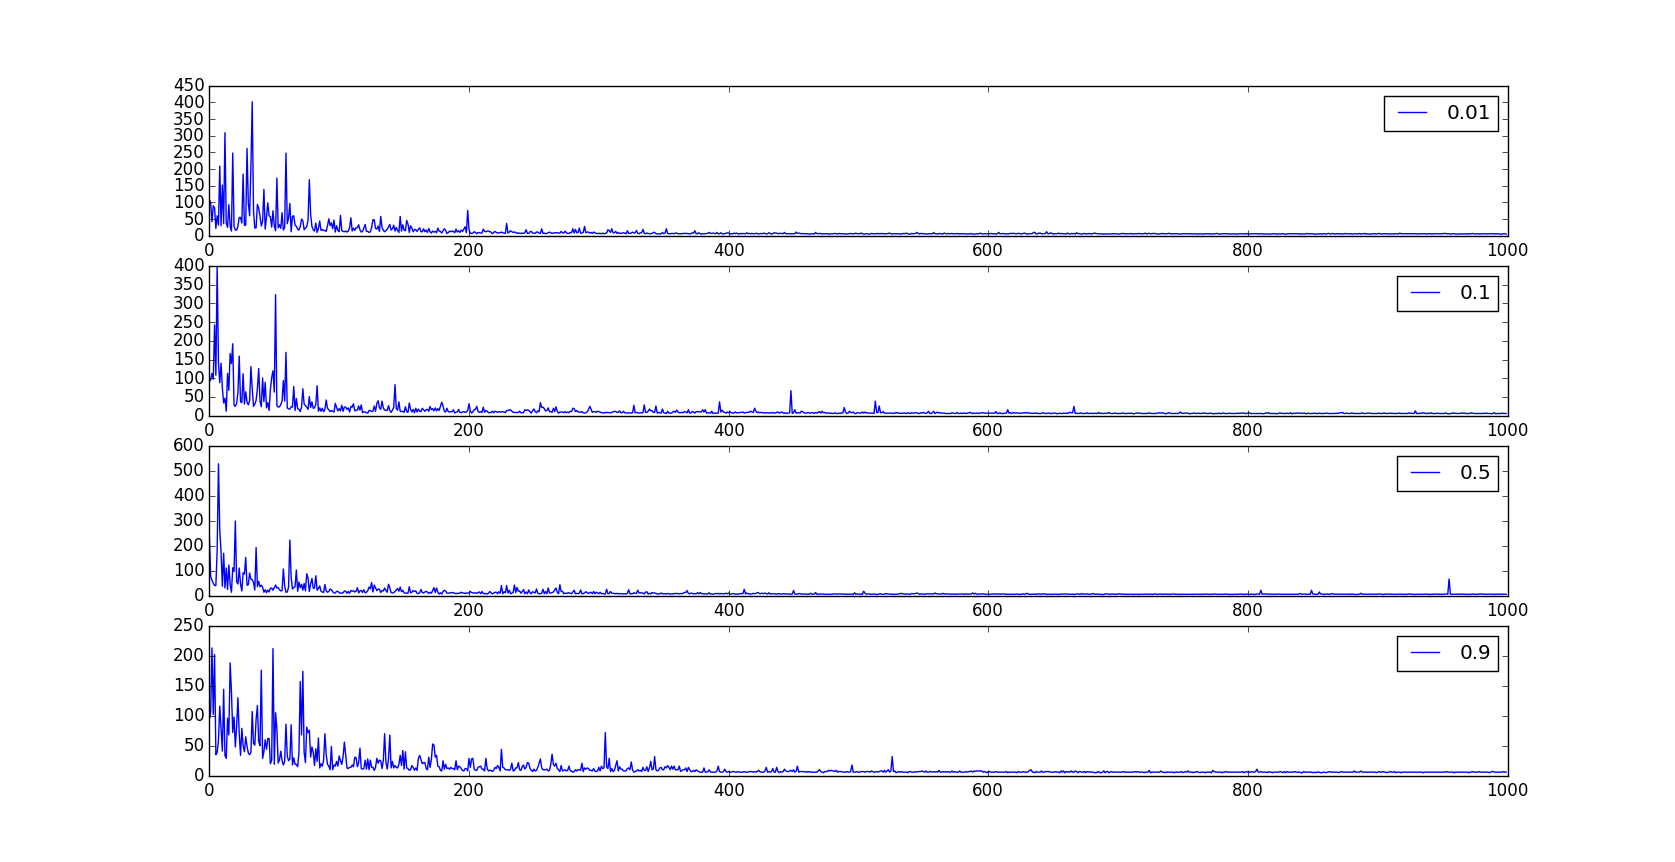
\includegraphics[scale=0.3]{allplots_hillclimbing}
	\captionof{figure}{Policy Hill-Climbing: 1 predator versus 1 prey, with varying step sizes}
	\label{graph:phc_1v1_steps}
\end{center}

The graph shows that all chosen step sizes start off quite radically. Eventually, all algorithms converge. The step size of 0.9 takes longest to stabilize and the highest number of rounds to catch the prey after stabilizing. As stated before, this high step size ensures a quite radical update of $\pi$. In this case, this parameter setting is not optimal. The lowest step size shows that $\pi$ changes gradually, but still quickly. Contrary to the larger step-sizes, this is quite stable for the lowest step size. All step sizes tend to have peaks in rounds needed to catch the prey, after stabilizing. The peaks at the lowest step size are smallest. Also, the number of rounds needed to catch the prey are lowest. Therefore, it seems that small step sizes are best.

\subsubsection{2 predators vs. 1 prey}
This section discusses what happens when two predators take on a prey.

\begin{center}
	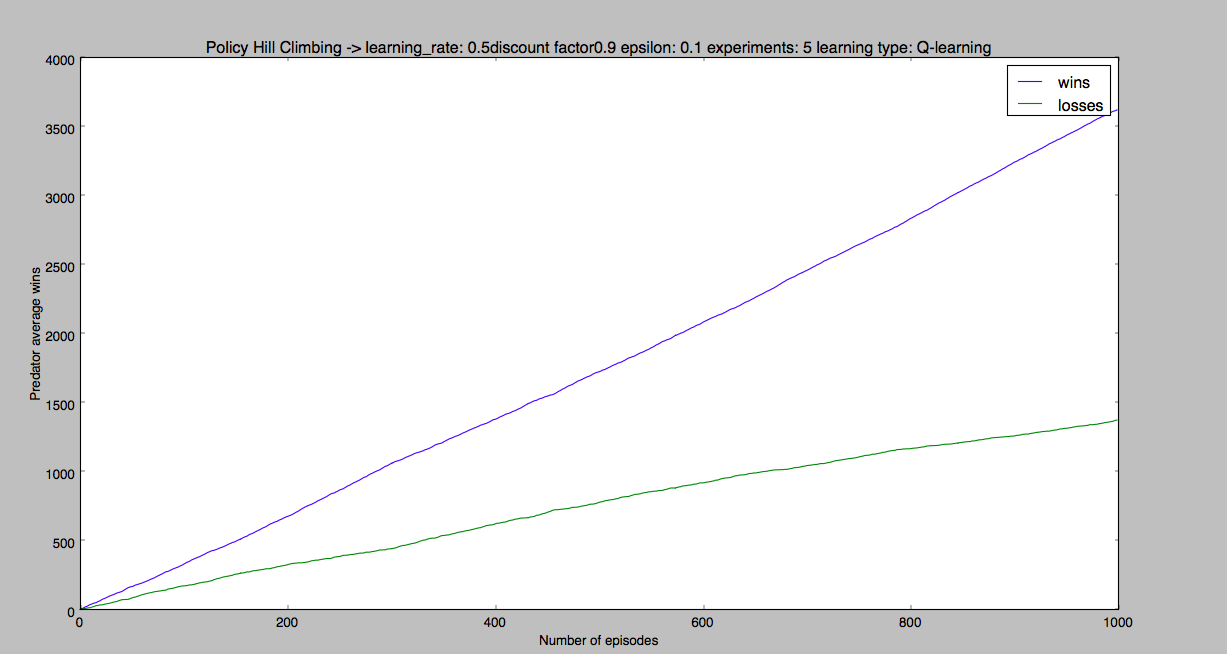
\includegraphics[scale=0.3]{hillclimbing1000times5step01}
	\captionof{figure}{Policy Hill-Climbing: 2 predators versus 1 prey}
	\label{graph:phc_2v1}
\end{center}

Graph \ref{graph:phc_2v1} shows that the predators win most episodes. As the number of losses by the predators decrease, it can be concluded that the predators are learning to cooperate and will continue to win most episodes. However, exploratory actions will lead to losses by the predators from time to time.

\begin{table}[H]
\begin{center}
\begin{tabular}{| l | l | l | l | l |}
\hline
 & \parbox{2cm}{\textbf{Avg wins \\ (first 100)}} & \parbox{2cm}{\textbf{Avg losses \\ (first 100)}} & \parbox{2cm}{\textbf{Avg wins \\ (last 100)}} & \parbox{2cm}{\textbf{Avg losses \\ (last 100)}} \\
\hline
\textbf{Predators} & 65 & 34 & 76 & 23 \\
\hline
\end{tabular}
\caption{Average number of rounds two predators need to catch one prey}
\label{table:phc_2vs1}
\end{center}
\end{table}

Table \ref{table:phc_2vs1} shows that the number of wins are indeed still increasing.

\subsubsection{3 predators vs. 1 prey}
Due to time constraints, this test was performed on a smaller grid. Other than that, all other parameters are set to default. 

\begin{center}
	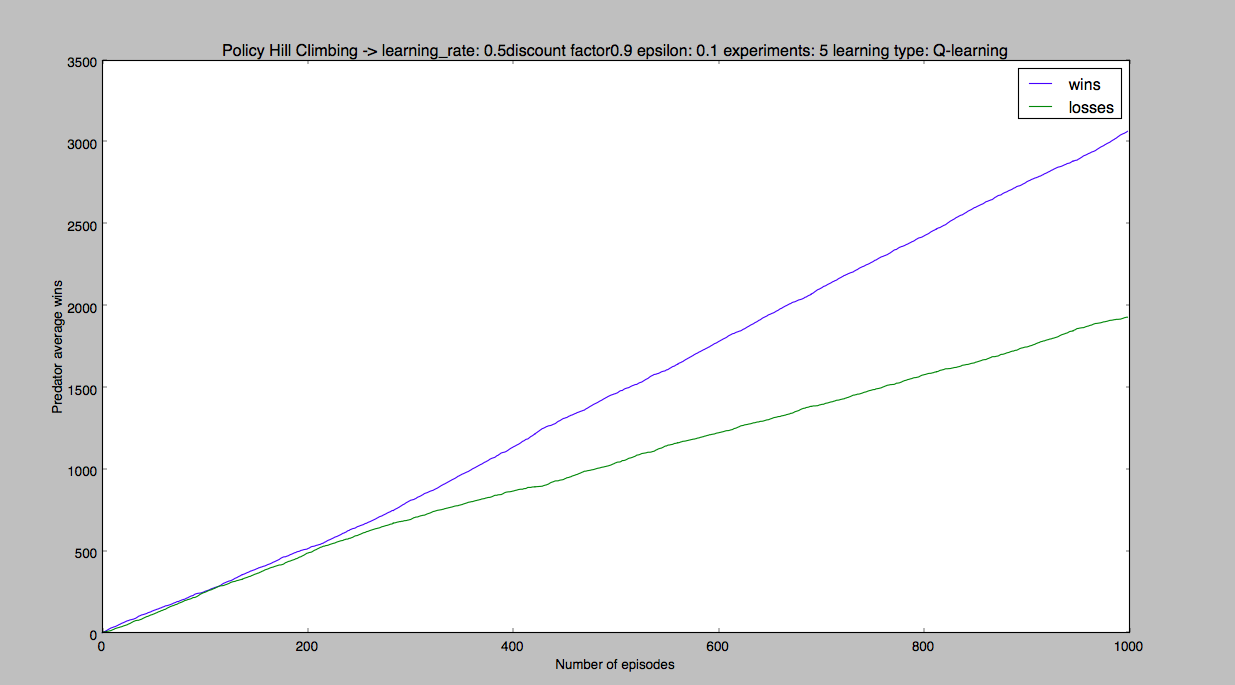
\includegraphics[scale=0.3]{phc_3predators_5by5_graph}
	\captionof{figure}{Policy Hill-Climbing: 3 predators versus 1 prey, on a 5x5 grid}
	\label{graph:phc_3v1}
\end{center}

The graph shows that the predators win more often than they lose. This shows that the policy hill-climbing performs better than independent Q-learning and independent SARSA.

\begin{table}[H]
\begin{center}
\begin{tabular}{| l | l | l | l | l |}
\hline
 & \parbox{2cm}{\textbf{Avg wins \\ (first 100)}} & \parbox{2cm}{\textbf{Avg losses \\ (first 100)}} & \parbox{2cm}{\textbf{Avg wins \\ (last 100)}} & \parbox{2cm}{\textbf{Avg losses \\ (last 100)}} \\
\hline
\textbf{Predators} & 50 & 62 & 62 & 36 \\
\hline
\end{tabular}
\caption{Average number of rounds two predators need to catch one prey}
\label{table:phc_3vs1}
\end{center}
\end{table}

The results in table \ref{table:phc_3vs1} shows that the predators are more and more successful in catching the prey. 